\section{Vecteurs gaussiens}

Vecteurs gaussiens are the one family of multivariate lois this course
handles in closed form, and two facts make that possible. The loi of a vecteur
gaussien is determined by two objects only, a mean vector and a matrice de
covariance, so every question about it reduces to linear algebra; and the family is
stable under every affine map, so the answer to such a question is again a
vecteur gaussien. What follows is the consequence of those two facts, together
with one counter-example showing that the definition which makes them true
cannot be weakened to the one a reader expects. Les vecteurs gaussiens
apparaissent également dans le théorème central limite, présenté au chapitre
suivant, as its limit.

\subsection{Rappels sur la loi normale}

Nous commençons par revoir les principales propriétés de la loi normale --- the
one-dimensional case, which chapter 4 introduced as a loi with a densité and
which this chapter needs in the sharper form of its fonction caractéristique.

\begin{definition}[Loi normale]
Une variable aléatoire réelle $X$ suit une loi normale d'espérance $\mu$ et de
variance $\sigma^{2}$, ce que l'on note $X \sim \mathcal{N}(\mu,\sigma^{2})$, si
elle a pour densité :
\[
  \forall x \in \reals, \qquad
  f_{X}(x) = \frac{1}{\sqrt{2\pi}\,\sigma}\,
             e^{-\frac{(x-\mu)^{2}}{2\sigma^{2}}} .
\]
Le paramètre $\sigma > 0$ est l'\textbf{écart type}
(\textit{standard deviation}) de $X$. La loi normale est également appelée
\textbf{loi gaussienne} (\textit{Gaussian distribution}), and the two names are
used interchangeably throughout.
\end{definition}

\begin{notation}
Par convention, on inclut dans les lois normales les mesures de Dirac. Ainsi une
mesure de Dirac en $\mu$ sera vue comme une loi normale d'espérance $\mu$ et
d'écart type $\sigma = 0$. Cette loi n'a évidemment pas de densité par rapport
à la mesure de Lebesgue, and the definition above does not cover
it --- it is a convention, not a theorem. It is kept because without it the
statements later in this chapter would each need a separate clause for the
dégénéré case: an affine image of a vecteur gaussien can be constant, a vecteur
gaussien with a singular matrice de covariance has components that are constant
along some direction, and in both cases the convention lets the result be stated
without an exception.
\end{notation}

Si $Z$ est une variable aléatoire suivant une loi normale centrée réduite, soit
$Z \sim \mathcal{N}(0,1)$, alors la variable aléatoire
\[
  X = \sigma Z + \mu
\]
suit une loi normale d'espérance $\mu$ et de variance $\sigma^{2}$. This
is the changement de variable computation of chapter 4, and it is the form in
which the loi normale is used here: everything Gaussian in this chapter is
built as an affine image of something centré réduit.

\begin{prop}[Fonction caractéristique de la loi normale]
La fonction caractéristique d'une variable aléatoire réelle $X$ suivant une loi
normale d'espérance $\mu$ et de variance $\sigma^{2}$ est donnée par :
\[
  \forall t \in \reals, \qquad
  \varphi_{X}(t) = e^{i\mu t}\, e^{-\frac{\sigma^{2}t^{2}}{2}} .
\]
\end{prop}

\begin{remark}
The loi normale centrée réduite case $\varphi_{Z}(t) = e^{-t^{2}/2}$ is the
differential-equation computation of chapter 6 --- differentiating under the
integral sign and integrating by parts shows that $\varphi_{Z}$ solves
$\varphi_{Z}'(t) = -t\,\varphi_{Z}(t)$ with $\varphi_{Z}(0) = 1$ --- and
everything else is the affine rule of that same chapter: writing $X = \sigma Z + \mu$ gives
$\varphi_{X}(t) = \expec\!\left(e^{it(\sigma Z + \mu)}\right)
 = e^{i\mu t}\varphi_{Z}(\sigma t) = e^{i\mu t}e^{-\sigma^{2}t^{2}/2}$.
The formula is also consistent with the Dirac convention: at $\sigma = 0$ it
reduces to $\varphi_{X}(t) = e^{i\mu t}$, which is the fonction caractéristique
of $\delta_{\mu}$.
\end{remark}

Two consequences are used constantly below. By chapter 6's Caractérisation de la loi, a
real variable is normal as soon as its fonction caractéristique has the shape
above --- one never has to produce a densité. And the exponent is a quadratic
polynomial in $t$, which makes the multivariate generalisation of the next
sections a matter of replacing $\sigma^{2}t^{2}$ by a quadratic form.

\subsection{Premier exemple}

Before any definition, one example says what the whole chapter is about.\\

Soit $X$, $Y$ deux variables aléatoires indépendantes suivant la loi normale
centrée réduite. Le vecteur aléatoire $(X,Y)$ a pour densité, by indépendance,
the product of the marginal densités:
\[
  \forall x,y \in \reals, \qquad
  f_{X,Y}(x,y) = f_{X}(x) f_{Y}(y)
               = \frac{1}{2\pi}\, e^{-\frac{x^{2}+y^{2}}{2}} .
\]
Sa fonction caractéristique est donnée par the product of the marginal
fonctions caractéristiques, again by indépendance:
\[
  \forall s,t \in \reals, \qquad
  \varphi_{X,Y}(s,t) = \varphi_{X}(s)\varphi_{Y}(t)
                     = e^{-\frac{s^{2}+t^{2}}{2}} .
\]

On s'intéresse à la projection orthogonale du vecteur aléatoire $(X,Y)$ sur le
vecteur unitaire $(\cos\theta,\sin\theta)$, avec $\theta \in [0,2\pi]$. On note
$S = X\cos\theta + Y\sin\theta$ leur produit scalaire. C'est une variable
aléatoire de fonction caractéristique, read off the joint one :
\[
  \forall t \in \reals, \qquad
  \varphi_{S}(t) = \expec\!\left(e^{it(X\cos\theta + Y\sin\theta)}\right)
                 = \varphi_{X,Y}(t\cos\theta,\, t\sin\theta)
                 = e^{-\frac{t^{2}(\cos^{2}\theta + \sin^{2}\theta)}{2}}
                 = e^{-\frac{t^{2}}{2}} .
\]
On en déduit que $S$ suit une loi normale --- the loi normale centrée réduite,
for every $\theta$. Ainsi la projection orthogonale du vecteur aléatoire $(X,Y)$
sur n'importe quel vecteur (même non unitaire) suit une loi normale: onto any
direction first, then, by scaling, onto any vector at all. That invariance is not
an accident of this pair: c'est une caractéristique des vecteurs gaussiens, and
the next section turns it into the definition.\\

The densité above depends on $(x,y)$ only through $x^{2}+y^{2}$, so its level
sets are circles. The figure below shows what happens to those level sets when
the two coordinates stop being independent and equally scaled: they become
ellipses, axis-aligned while the matrice de covariance is diagonal and rotated as
soon as the off-diagonal term is non-zero. Nothing else changes --- the level
sets of a bivariate Gaussian densité are always ellipses, which is what a
quadratic form in the exponent means.

\begin{figure}[ht]
\centering
\begin{tikzpicture}[scale=0.78]
  \draw[->] (-2.5,0) -- (2.5,0) node[right,font=\scriptsize] {$x_{1}$};
  \draw[->] (0,-2.5) -- (0,2.5) node[above,font=\scriptsize] {$x_{2}$};
  \foreach \r in {0.65,1.3,1.95} \draw[blue!65!black,thick] (0,0) circle (\r);
  \node[font=\scriptsize] at (0,-3.15)
    {$\Gamma = \left(\begin{smallmatrix} 1 & 0 \\ 0 & 1 \end{smallmatrix}\right)$};
  \node[font=\scriptsize] at (0,-3.85) {circles};
\end{tikzpicture}
\hspace{0.7cm}
\begin{tikzpicture}[scale=0.78]
  \draw[->] (-2.5,0) -- (2.5,0) node[right,font=\scriptsize] {$x_{1}$};
  \draw[->] (0,-2.5) -- (0,2.5) node[above,font=\scriptsize] {$x_{2}$};
  \foreach \k in {0.65,1.3,1.95}
    \draw[blue!65!black,thick] (0,0) ellipse ({1.30*\k} and {0.55*\k});
  \node[font=\scriptsize] at (0,-3.15)
    {$\Gamma = \left(\begin{smallmatrix} 1.7 & 0 \\ 0 & 0.3 \end{smallmatrix}\right)$};
  \node[font=\scriptsize] at (0,-3.85) {axis-aligned};
\end{tikzpicture}
\hspace{0.7cm}
\begin{tikzpicture}[scale=0.78]
  \draw[->] (-2.5,0) -- (2.5,0) node[right,font=\scriptsize] {$x_{1}$};
  \draw[->] (0,-2.5) -- (0,2.5) node[above,font=\scriptsize] {$x_{2}$};
  \foreach \k in {0.65,1.3,1.95}
    \draw[blue!65!black,thick,rotate=45] (0,0) ellipse ({1.34*\k} and {0.45*\k});
  \draw[gray,dashed] (-2.1,-2.1) -- (2.1,2.1);
  \node[font=\scriptsize] at (0,-3.15)
    {$\Gamma = \left(\begin{smallmatrix} 1 & 0.8 \\ 0.8 & 1 \end{smallmatrix}\right)$};
  \node[font=\scriptsize] at (0,-3.85) {rotated};
\end{tikzpicture}

\vspace{0.9cm}

{\centering \small \textit{Level sets of a centrée bivariate Gaussian densité at
three matrices de covariance. The axes of the ellipses are the eigenvectors of
$\Gamma$ and their half-lengths are proportional to the square roots of its
eigenvalues; the dashed line in the third panel is the direction of largest
variance, which rotates away from the coordinate axes exactly when the
off-diagonal term is non-zero.}\par}
\end{figure}

\subsection{Définition}

Soit $n \geq 1$ un entier.

\begin{definition}[Vecteur gaussien]
Un vecteur aléatoire $X$ de dimension $n$ est un \textbf{vecteur gaussien}
(\textit{Gaussian vector}) si pour tout $a \in \reals^{n}$, la variable
aléatoire réelle $a^{T}X$ suit une loi gaussienne.
\end{definition}

Read that once more, because it is the whole chapter. The condition is on
\emph{every} linear combination of the components, not on the components. It is
not the definition a reader expects, which would be:

\begin{center}
\emph{(wrong)} $X$ is a vecteur gaussien when each component $X_{1},\dots,X_{n}$
follows a loi normale.
\end{center}

That condition is strictly weaker. It is implied by the real definition --- take
$a$ to be the $i$-th unit vector and $a^{T}X = X_{i}$ --- but it does not imply
it, and the counter-example below exhibits a pair of variables of loi normale
centrée réduite whose loi jointe is not Gaussian. Everything this chapter proves
is false under the weaker condition, so the distinction is not pedantry: it is
the hypothesis every theorem below is checked against.\\

Un vecteur gaussien a nécessairement une espérance et une matrice de covariance.
Il suffit de prendre pour $a$ les vecteurs unitaires de $\reals^{n}$: that makes
each component a normal variable, and a normal variable has moments of every
order, so no integrability hypothesis ever has to be added to a statement about
vecteurs gaussiens. Si $X$ est un vecteur gaussien d'espérance $\mu$ et de
matrice de covariance $\Gamma$, alors pour tout $a \in \reals^{n}$, la variable
aléatoire $a^{T}X$ suit une loi gaussienne d'espérance et de variance :
\[
  \expec(a^{T}X) = a^{T}\mu, \qquad
  \Var(a^{T}X) = \Cov(a^{T}X, a^{T}X) = a^{T}\Cov(X)\,a = a^{T}\Gamma a .
\]
In particular $a^{T}\Gamma a \geq 0$ for every $a$: the matrice de covariance of
a vecteur gaussien is symétrique and positive semi-definite, as any matrice de
covariance is. It need not be invertible, and the densité section below is about
what invertibility buys.

\begin{theorem}[Fonction caractéristique d'un vecteur gaussien]
Un vecteur gaussien $X$ d'espérance $\mu$ et de matrice de covariance $\Gamma$ a
pour fonction caractéristique :
\[
  \forall t \in \reals^{n}, \qquad
  \varphi_{X}(t) = e^{it^{T}\mu}\, e^{-\frac{t^{T}\Gamma t}{2}} .
\]
\end{theorem}

\begin{remark}
One line, and it is the reason the definition is stated over all linear
combinations. Pour tout $t \in \reals^{n}$, la variable aléatoire $t^{T}X$ suit
une loi gaussienne d'espérance $t^{T}\mu$ et de variance $t^{T}\Gamma t$, by
definition, so evaluating its one-dimensional fonction caractéristique at the
single point $1$ gives
\[
  \varphi_{X}(t) = \expec\!\left(e^{it^{T}X}\right) = \varphi_{t^{T}X}(1)
                 = e^{it^{T}\mu}e^{-\frac{t^{T}\Gamma t}{2}} ,
\]
the last equality being the proposition above on the fonction caractéristique
de la loi normale. A definition by lois marginales
would give this at the $n$ unit vectors only, which is not enough to know the
joint fonction caractéristique.
\end{remark}

\begin{notation}
Since the fonction caractéristique determines the loi, la loi d'un vecteur
gaussien est entièrement caractérisée par son espérance et sa matrice de
covariance. On notera $X \sim \mathcal{N}(\mu,\Gamma)$ un vecteur gaussien
d'espérance $\mu$ et de matrice de covariance $\Gamma$. The reuse of the symbol
$\Gamma$ here is one of the deliberate collisions chapter 2 sets out.
\end{notation}

This is the practical content of the chapter. To identify the loi of
anything built from a vecteur gaussien, it suffices to check that the thing is
Gaussian and then to compute two objects, a mean vector and a matrice de
covariance. No densité, no integral, no convolution.

\begin{example}[Reading off the loi of a projection]
Soit $X$ un vecteur gaussien, with
\[
  \mu = \begin{pmatrix} 2 \\ 1 \end{pmatrix}, \qquad
  \Gamma = \begin{pmatrix} 2 & -1 \\ -1 & 3 \end{pmatrix}, \qquad
  a = \begin{pmatrix} 1 \\ -1 \end{pmatrix} .
\]
The variable $a^{T}X = X_{1} - X_{2}$ est une variable aléatoire de loi
gaussienne, comme projection d'un vecteur gaussien --- by definition --- so only
its two parameters are left to compute:
\[
  \expec(a^{T}X) = a^{T}\mu = 2 - 1 = 1, \qquad
  \Var(a^{T}X) = a^{T}\Gamma a = 2 - (-1) - (-1) + 3 = 7 .
\]
Hence $a^{T}X \sim \mathcal{N}(1,7)$. The whole computation is the expansion
$a^{T}\Gamma a = \Gamma_{11} - \Gamma_{12} - \Gamma_{21} + \Gamma_{22}$, and the
two off-diagonal terms are counted twice precisely because $\Gamma$ is symétrique.
\end{example}

\subsection{Construction d'un vecteur gaussien}

Soit $Z$ un vecteur aléatoire dont les composantes sont $n$ variables aléatoires
i.i.d.\ de loi normale centrée réduite. Il est facile de voir que $Z$ est un
vecteur gaussien, by indépendance :
\[
  \forall t \in \reals^{n}, \qquad
  \varphi_{Z}(t) = \expec\!\left(e^{it^{T}Z}\right)
                 = \varphi_{Z_{1}}(t_{1}) \dots \varphi_{Z_{n}}(t_{n})
                 = e^{-\frac{\|t\|^{2}}{2}} ,
\]
which is the fonction caractéristique of the previous section with $\mu = 0$ and
$\Gamma = I_{n}$. L'espérance de $Z$ est nulle et sa matrice de covariance est la
matrice identité : sa loi est dite \textbf{centrée réduite}
(\textit{standard}).
Les transformations affines de $Z$ permettent de construire n'importe quel
vecteur gaussien.

\begin{prop}
Pour toute matrice $A$ de taille $n \times n$ et tout vecteur $\mu$ de dimension
$n$, le vecteur aléatoire $X = AZ + \mu$ est un vecteur gaussien d'espérance
$\mu$ et de matrice de covariance $\Gamma = AA^{T}$.
\end{prop}

\begin{remark}
Pour tout $a \in \reals^{n}$, la variable aléatoire
$a^{T}X = (A^{T}a)^{T}Z + a^{T}\mu$, qui est la projection d'un vecteur
gaussien, suivie d'une translation, suit une loi gaussienne. Le vecteur aléatoire
$X$ est donc gaussien, by definition. Son espérance et sa matrice de covariance
sont données par
$\expec(X) = A\expec(Z) + \mu = \mu$ and
$\Cov(X) = \Cov(AZ) = A\Cov(Z)A^{T} = AA^{T}$, by linearity of the espérance and
bilinearity of the covariance.
\end{remark}

\begin{remark}
The construction reaches every vecteur gaussien, not just some. A matrice de
covariance $\Gamma$ is symétrique and positive semi-definite, so it has a spectral
decomposition $\Gamma = UDU^{T}$ with $U$ orthogonal and $D$ diagonal with
non-negative entries; taking $A = UD^{1/2}$ gives $AA^{T} = \Gamma$. So for every
$\mu$ and every symétrique positive semi-definite $\Gamma$ there is a vecteur
gaussien $\mathcal{N}(\mu,\Gamma)$, and it can always be realised as $AZ + \mu$
with $Z$ centré réduit. Positive semi-definiteness is the whole condition --- a
symétrique matrix that fails it is not the matrice de covariance of anything.
\end{remark}

\begin{example}[Which matrices de covariance are admissible]
Soit $X$ un vecteur gaussien centré de dimension $2$ et de matrice de covariance
\[
  \Gamma = \begin{pmatrix} 1 & 1 \\ 1 & \alpha \end{pmatrix} .
\]
For $\Gamma$ to be a matrice de covariance, la matrice doit être semi-définie
positive. A symétrique $2 \times 2$ matrix is positive semi-definite exactly when
its two diagonal entries and its determinant are all non-negative. Here those
three quantities are $\Gamma_{11} = 1$, $\Gamma_{22} = \alpha$ and
$\det\Gamma = \alpha - 1$, so the conditions read $\alpha \geq 0$ together with
$\alpha \geq 1$, and il faut et il suffit d'avoir $\alpha \geq 1$ --- the
determinant condition is the binding one and it subsumes the condition on the
second diagonal entry. The boundary case $\alpha = 1$ is the dégénéré
one: there $\det\Gamma = 0$, the vector is carried by a line, and the densité
theorem below says it has no densité. For $\alpha > 1$ it does, and les
composantes ne sont pas indépendantes, whatever $\alpha$ is, since the
off-diagonal entry is $1 \neq 0$ --- leur coefficient de corrélation est
$1/(\sqrt{1}\sqrt{\alpha}) = 1/\sqrt{\alpha}$, which tends to $0$ but never
reaches it.
\end{example}

\subsection{Un contre-exemple}

Les composantes d'un vecteur gaussien suivent des lois gaussiennes : il suffit de
projeter le vecteur sur chaque vecteur unitaire de $\reals^{n}$. La réciproque
n'est pas vraie. Nous donnons ici un exemple de vecteur aléatoire dont les
composantes suivent des lois gaussiennes mais qui n'est pas gaussien. It is the
reason the definition above is stated over all linear combinations, and it is
worth carrying with its computation rather than as an assertion, because the
computation is short and because the same shape recurs.\\

Soit $Z$ une variable aléatoire suivant une loi normale centrée réduite et $Y$
une variable aléatoire discrète, indépendante de $Z$, qui vaut $1$ avec
probabilité $\tfrac{1}{2}$ et $-1$ sinon. On vérifie facilement que $YZ$ suit une
loi gaussienne. Conditioning on the two values of $Y$ and using indépendance,
\[
  \forall t \in \reals, \qquad
  \varphi_{YZ}(t) = \expec\!\left(e^{iYZt}\right)
                  = \tfrac{1}{2}\expec\!\left(e^{iZt}\right)
                    + \tfrac{1}{2}\expec\!\left(e^{-iZt}\right)
                  = \tfrac{1}{2}\varphi_{Z}(t) + \tfrac{1}{2}\varphi_{Z}(-t)
                  = \varphi_{Z}(t) ,
\]
the last equality because $\varphi_{Z}(t) = e^{-t^{2}/2}$ is even. By injectivity
of the fonction caractéristique, $YZ \sim \mathcal{N}(0,1)$.\\

Le vecteur $X = (Z, YZ)$, dont les composantes suivent des lois gaussiennes (both
of them the loi normale centrée réduite), n'est pas gaussien. En effet, sa
projection sur le vecteur $a = (1,1)$ --- the variable $a^{T}X = Z + YZ$ ---
satisfies
\[
  \prob(Z + YZ = 0) = \prob(Y = -1) = \tfrac{1}{2} ,
\]
since $Z + YZ = 0$ on the événement $\{Y = -1\}$. A loi normale can put mass
$\tfrac{1}{2}$ on a single point only if it is a Dirac mass, that is only if
$\sigma = 0$ under the Dirac convention above; and $Z + YZ$ is not presque
sûrement $0$, because on the événement $\{Y = 1\}$, of probability $\tfrac{1}{2}$,
it equals $2Z \sim \mathcal{N}(0,4)$. So $Z + YZ$ is neither a variable with a
normal densité nor a Dirac mass, hence not normal, hence $X$ is not a vecteur
gaussien.\\

Pour qu'un vecteur aléatoire dont les composantes suivent des lois gaussiennes
soit gaussien, il faut des conditions supplémentaires, comme l'indépendance de
ses composantes, as the concatenation corollary below shows.

\begin{remark}
The same pair says something sharper, and it is the reason to keep it in view
when reading the indépendance theorem below. The two components are
\emph{décorrélées}:
\[
  \Cov(Z, YZ) = \expec(Z \cdot YZ) - \expec(Z)\expec(YZ)
              = \expec(Y)\expec(Z^{2}) - 0 = 0 ,
\]
using the indépendance of $Y$ and $Z$ and $\expec(Y) = 0$. They are very far from
independent, since $|YZ| = |Z|$ makes each one a function of the other's absolute
value. Two variables of loi normale centrée réduite, décorrélées, not
independent. Nothing is wrong: the indépendance theorem below, the one that turns
zero covariance into indépendance, has the hypothesis that the pair is a vecteur
gaussien, and this pair is not.
\end{remark}

\begin{figure}[ht]
\centering
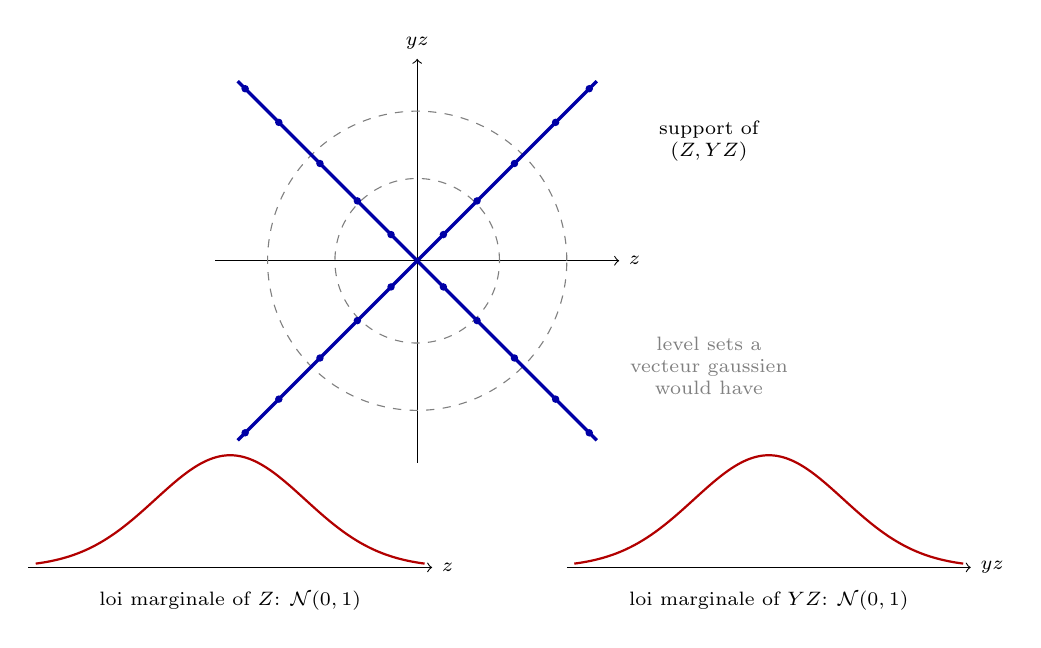
\begin{tikzpicture}[scale=0.95]
  \draw[->] (-2.7,0) -- (2.7,0) node[right,font=\scriptsize] {$z$};
  \draw[->] (0,-2.7) -- (0,2.7) node[above,font=\scriptsize] {$yz$};
  \draw[gray,dashed] (0,0) circle (1.1);
  \draw[gray,dashed] (0,0) circle (2.0);
  \draw[very thick,blue!65!black] (-2.4,-2.4) -- (2.4,2.4);
  \draw[very thick,blue!65!black] (-2.4,2.4) -- (2.4,-2.4);
  \foreach \s in {0.35,0.8,1.3,1.85,2.3}
    {\fill[blue!65!black] (\s,\s) circle (0.05);
     \fill[blue!65!black] (-\s,-\s) circle (0.05);
     \fill[blue!65!black] (\s,-\s) circle (0.05);
     \fill[blue!65!black] (-\s,\s) circle (0.05);}
  \node[font=\scriptsize,align=center] at (3.9,1.6)
    {support of\\$(Z,YZ)$};
  \node[font=\scriptsize,align=center,gray] at (3.9,-1.4)
    {level sets a\\vecteur gaussien\\would have};
  \begin{scope}[xshift=-2.5cm,yshift=-4.1cm]
    \draw[->] (-2.7,0) -- (2.7,0) node[right,font=\scriptsize] {$z$};
    \draw[thick,red!70!black,smooth,samples=80,domain=-2.6:2.6]
      plot (\x,{1.5*exp(-\x*\x/2)});
    \node[font=\scriptsize] at (0,-0.45) {loi marginale of $Z$: $\mathcal{N}(0,1)$};
  \end{scope}
  \begin{scope}[xshift=4.7cm,yshift=-4.1cm]
    \draw[->] (-2.7,0) -- (2.7,0) node[right,font=\scriptsize] {$yz$};
    \draw[thick,red!70!black,smooth,samples=80,domain=-2.6:2.6]
      plot (\x,{1.5*exp(-\x*\x/2)});
    \node[font=\scriptsize] at (0,-0.45) {loi marginale of $YZ$: $\mathcal{N}(0,1)$};
  \end{scope}
\end{tikzpicture}

{\centering \small \textit{The counter-example. Both lois marginales are the bell
curve of the loi normale centrée réduite, yet the loi jointe sits on the union of
the two diagonals and is visibly not elliptical --- it is carried by a set
négligeable pour la mesure de Lebesgue, so it has no densité at all. The dashed
circles show the level sets the loi jointe would have had if the pair were a
vecteur gaussien with these lois marginales and zero covariance.}\par}
\end{figure}

\subsection{Existence d'une densité}

A vecteur gaussien always has a loi, a fonction caractéristique and
moments of every order. Whether it has a \emph{densité} is a separate question,
and the answer is a single linear-algebra condition.

\begin{theorem}[Densité d'un vecteur gaussien]
Un vecteur gaussien $X$ d'espérance $\mu$ et de matrice de covariance $\Gamma$ a
une densité par rapport à la mesure de Lebesgue si et seulement si $\Gamma$ est
inversible. Cette densité est alors donnée par :
\[
  \forall x \in \reals^{n}, \qquad
  f_{X}(x) = \frac{1}{(2\pi)^{\frac{n}{2}}\sqrt{\det\Gamma}}\,
             e^{-\frac{1}{2}(x-\mu)^{T}\Gamma^{-1}(x-\mu)} .
\]
\end{theorem}

\begin{proof}
Comme $\Gamma$ est symétrique et positive, il existe une matrice $A$ de taille
$n \times n$ telle que $\Gamma = AA^{T}$. By the previous section, on peut donc
écrire $X = AZ + \mu$ avec $Z$ un vecteur gaussien centré réduit de dimension
$n$. Ce vecteur a pour densité :
\[
  \forall z \in \reals^{n}, \qquad
  f_{Z}(z) = \frac{1}{(2\pi)^{\frac{n}{2}}}\, e^{-\frac{\|z\|^{2}}{2}} .
\]
By the théorème de transfert, pour toute fonction mesurable positive $\phi$, on
a :
\[
  \expec(\phi(X)) = \expec(\phi(AZ + \mu))
    = \int \phi(Az + \mu)\, \frac{1}{(2\pi)^{\frac{n}{2}}}\,
      e^{-\frac{\|z\|^{2}}{2}}\, dz .
\]

Si $\Gamma$ est inversible, $A$ l'est aussi, since $\det\Gamma = (\det A)^{2}$,
et l'application $z \mapsto Az + \mu$ est un difféomorphisme de $\reals^{n}$ onto
itself, de matrice jacobienne $A$, which is constant. On obtient par changement
de variable $x = Az + \mu$, whose inverse is $z = A^{-1}(x-\mu)$ and whose
Jacobian factor is $|\det A|$ :
\[
  \expec(\phi(X)) = \int \phi(x)\, \frac{1}{(2\pi)^{\frac{n}{2}}}\,
    e^{-\frac{1}{2}(x-\mu)^{T}(A^{-1})^{T}A^{-1}(x-\mu)}\,
    \frac{dx}{|\det A|} .
\]
Now $(A^{-1})^{T}A^{-1} = (AA^{T})^{-1} = \Gamma^{-1}$ and
$|\det A| = \sqrt{\det\Gamma}$; on en déduit le résultat attendu --- the
integrand is the announced densité and $X$ has that densité, the function $\phi$
being an arbitrary positive mesurable fonction test.\\

Si $\Gamma$ n'est pas inversible, $A$ ne l'est pas non plus et il existe un
vecteur $u \in \reals^{n}$ non nul tel que $u^{T}A = 0$. For that
$u$,
\[
  u^{T}(X - \mu) = u^{T}AZ = 0 \qquad \text{almost surely}, \qquad \text{hence}
  \qquad \prob\!\left(u^{T}(X-\mu) = 0\right) = 1 .
\]
L'hyperplan $\{x \in \reals^{n} : u^{T}(x - \mu) = 0\}$ de $\reals^{n}$ est
négligeable pour la mesure de Lebesgue. A vecteur aléatoire with a densité gives
probability zero to every set négligeable pour la mesure de Lebesgue, so le
vecteur $X$ ne peut avoir de densité.
\end{proof}

The second half of the proof is not a technicality to be skipped, and the vectors
it describes are not error cases. When $\Gamma$ is singular of rank $r < n$, the
vector $X$ is carried by the affine subspace $\mu + \operatorname{im}(A)$ of
dimension $r$: it is a genuine vecteur gaussien, its fonction caractéristique is
still $e^{it^{T}\mu}e^{-t^{T}\Gamma t/2}$, its loi is still determined by
$\mu$ and $\Gamma$, and along the $n-r$ directions in the kernel it is deterministic.
Such a vector is called \textbf{dégénéré} (\textit{degenerate}). It simply has no
densité on $\reals^{n}$ --- though it does have one on the subspace that carries
it, once that subspace is identified with $\reals^{r}$. Vecteurs gaussiens
dégénérés turn up on their own in exam problems, most often as a residual vector
after a projection, so the right reflex on being asked for a densité is to
compute $\det\Gamma$ first.

\begin{figure}[ht]
\centering
\begin{tikzpicture}[scale=1.05]
  \draw[->] (-1.2,0) -- (3.3,0) node[right,font=\scriptsize] {$x_{1}$};
  \draw[->] (0,-1.2) -- (0,3.3) node[above,font=\scriptsize] {$x_{2}$};
  \draw[very thick,blue!65!black] (-0.9,2.9) -- (2.9,-0.9);
  \foreach \s in {-1.3,-0.85,-0.45,0.45,0.85,1.3}
    \draw[blue!65!black,fill=white,thin]
      ({1+0.707*\s},{1-0.707*\s}) circle (0.065);
  \fill[red!75!black] (1,1) circle (0.085);
  \node[font=\scriptsize,red!75!black,anchor=west] at (1.25,1.35) {$\mu = (1,1)$};
  \draw[->,gray,thick] (1,1) -- (1.75,0.25);
  \node[font=\scriptsize,gray,anchor=west] at (1.85,0.55) {$\operatorname{im}(A)$};
  \node[font=\scriptsize,align=left,anchor=west] at (0.4,2.9)
    {$X = (W+1,\, 1-W)$, \ $W \sim \mathcal{N}(0,1)$\\[2pt]
     $\Gamma = \left(\begin{smallmatrix} 1 & -1 \\ -1 & 1 \end{smallmatrix}\right)$,
     \ $\det\Gamma = 0$};
\end{tikzpicture}

{\centering \small \textit{A vecteur gaussien dégénéré in $\reals^{2}$: all its
mass lies on the line $x_{1} + x_{2} = 2$, which is négligeable pour la mesure de
Lebesgue, so there is no densité on the plane. The loi is still Gaussian, still
determined by $\mu$ and $\Gamma$, and on the line itself it is a one-dimensional
$\mathcal{N}(0,2)$ about $\mu$.}\par}
\end{figure}

\begin{example}[Two vectors built from one normal variable]
Soit $W \sim \mathcal{N}(0,1)$ une variable aléatoire de loi normale centrée
réduite --- a single one. The vector
$(W, 2W, 3W)$ is Gaussian: any linear combination
$a_{1}W + 2a_{2}W + 3a_{3}W = (a_{1}+2a_{2}+3a_{3})W$ is a scalar multiple of
$W$, hence normal --- including the case where the scalar vanishes, which is the
Dirac mass at $0$ and is normal by convention. Its mean is $0$ and its matrice
de covariance is
\[
  \Gamma = \begin{pmatrix} 1 & 2 & 3 \\ 2 & 4 & 6 \\ 3 & 6 & 9 \end{pmatrix} ,
\]
of rank $1$, hence singular: no densité. The vector lives on the line spanned by
$(1,2,3)$, which is what rank $1$ says.\\

The vector $(W+1, 1-W)$ is Gaussian for the same reason, with mean $(1,1)$ and
matrice de covariance
\[
  \Gamma = \begin{pmatrix} 1 & -1 \\ -1 & 1 \end{pmatrix} ,
  \qquad \det\Gamma = 0 .
\]
Again no densité: the two components sum to $2$ presque sûrement, so the vector
is carried by the line $x_{1} + x_{2} = 2$. This is the vector drawn in the
figure above.
\end{example}

\begin{example}[Recognising a vecteur gaussien from its densité]
Soit $(X,Y)$ un vecteur aléatoire de densité :
\[
  \forall x,y \in \reals, \qquad
  f_{X,Y}(x,y) = c\,\exp\!\left(-\tfrac{1}{8}\left(3x^{2} + 2xy + 3y^{2}\right)\right) ,
\]
avec $c$ une constante strictement positive. The exponent is a negative definite
quadratic form with no linear part, so the theorem above identifies the
loi by matching coefficients: the vector is a vecteur gaussien centré with
\[
  \tfrac{1}{2}\begin{pmatrix} x \\ y \end{pmatrix}^{T} \Gamma^{-1}
  \begin{pmatrix} x \\ y \end{pmatrix}
  = \tfrac{1}{8}\left(3x^{2} + 2xy + 3y^{2}\right)
  \quad\Longrightarrow\quad
  \Gamma^{-1} = \tfrac{1}{4}\begin{pmatrix} 3 & 1 \\ 1 & 3 \end{pmatrix} ,
\]
the off-diagonal entries of $\Gamma^{-1}$ each carrying half of the cross term
$2xy$ because the form is symétrique. Inverting,
\[
  \Gamma = 4 \cdot \frac{1}{8}\begin{pmatrix} 3 & -1 \\ -1 & 3 \end{pmatrix}
         = \frac{1}{2}\begin{pmatrix} 3 & -1 \\ -1 & 3 \end{pmatrix},
  \qquad \det\Gamma = \frac{9-1}{4} = 2 ,
\]
so the normalising constant is forced:
$c = 1/\left(2\pi\sqrt{\det\Gamma}\right) = 1/(2\pi\sqrt{2})$. The lois
marginales are read off the diagonal, $X \sim \mathcal{N}(0,\tfrac{3}{2})$ and
$Y \sim \mathcal{N}(0,\tfrac{3}{2})$, and the components are not independent
since $\Gamma$ is not diagonal --- their coefficient de corrélation is
$(-\tfrac{1}{2})/(\tfrac{3}{2}) = -\tfrac{1}{3}$.
\end{example}

\subsection{Propriétés}

Nous terminons par quelques propriétés utiles des vecteurs gaussiens --- the
properties that do the work in practice. The first is the one almost every
exercise on this chapter starts from.

\begin{theorem}[Transformation affine]
Toute transformation affine d'un vecteur gaussien est un vecteur gaussien.
Precisely, if $X \sim \mathcal{N}(\mu,\Gamma)$ has dimension $n$, avec $A$
matrice de taille $m \times n$ et $b$ vecteur de dimension $m$, then
\[
  Y = AX + b \ \sim\ \mathcal{N}\!\left(A\mu + b,\ A\Gamma A^{T}\right) .
\]
\end{theorem}

\begin{remark}
The fonction caractéristique computes itself, and the computation is where the
transformed parameters come from:
\[
  \varphi_{Y}(t) = \expec\!\left(e^{it^{T}(AX+b)}\right)
                 = e^{it^{T}b}\,\varphi_{X}(A^{T}t)
                 = e^{it^{T}(A\mu + b)}\, e^{-\frac{1}{2}t^{T}A\Gamma A^{T}t} ,
\]
for $t \in \reals^{m}$. Il s'agit de la fonction caractéristique d'un vecteur
gaussien d'espérance $A\mu + b$ et de matrice de covariance $A\Gamma A^{T}$. Note
that $A$ need not be square and need not have full rank: $m$ may exceed $n$ or
fall short of it, and $A\Gamma A^{T}$ is then very often singular. That is fine,
and it is why the dégénéré case of the densité section had to be kept.
\end{remark}

This theorem is the workhorse. Any question of the form ``what is the
loi of this linear combination, this projection, this residual'' is
answered by writing the object as $AX + b$ and computing $A\mu + b$ and $A\Gamma A^{T}$.

\begin{theorem}[Indépendance des composantes]
Les composantes d'un vecteur gaussien sont indépendantes si et seulement si la
matrice de covariance de ce vecteur est diagonale.
\end{theorem}

\begin{remark}
By the fonction caractéristique theorem above, un vecteur gaussien $X$
d'espérance $\mu$ et de matrice de covariance $\Gamma$ a pour fonction
caractéristique $\varphi_{X}(t) = e^{it^{T}\mu}e^{-t^{T}\Gamma t/2}$. Chapter 6's
criterion says les composantes sont indépendantes si et seulement si cette
fonction s'écrit comme un produit of functions of the individual $t_{i}$. The
linear part $e^{it^{T}\mu}$ always
factorises; the quadratic part $t^{T}\Gamma t = \sum_{j,k}\Gamma_{jk}t_{j}t_{k}$
factorises exactly when it has no cross term, that is exactly when $\Gamma$ is
diagonal.
\end{remark}

\begin{remark}
Deux composantes d'un vecteur gaussien sont indépendantes si et seulement si leur
covariance est nulle. Il suffit en effet d'appliquer le résultat précédent au
vecteur aléatoire formé par ces deux composantes, qui est lui-même gaussien by
the affine transformation theorem --- extracting two coordinates is a linear map.
\end{remark}

\begin{remark}
The same computation covers \textbf{blocs} (\textit{blocks}), which is the form
used in the examples below. Split a vecteur gaussien $X$ into blocs
$X^{(1)},\dots,X^{(p)}$ of dimensions $n_{1},\dots,n_{p}$ and split $t$ the same
way. If $\Gamma$ is diagonal by blocs for that split, with diagonal blocs
$\Gamma^{(1)},\dots,\Gamma^{(p)}$ --- the diagonal blocs themselves being
arbitrary --- then
$t^{T}\mu = \sum_{k}(t^{(k)})^{T}\mu^{(k)}$ and
$t^{T}\Gamma t = \sum_{k}(t^{(k)})^{T}\Gamma^{(k)}t^{(k)}$, so
\[
  \varphi_{X}(t) = \prod_{k=1}^{p}
    e^{i(t^{(k)})^{T}\mu^{(k)}}\,
    e^{-\frac{1}{2}(t^{(k)})^{T}\Gamma^{(k)}t^{(k)}}
  = \prod_{k=1}^{p} \varphi_{X^{(k)}}\!\left(t^{(k)}\right) ,
\]
each factor being the fonction caractéristique of the bloc $X^{(k)}$, which is
Gaussian with mean $\mu^{(k)}$ and matrice de covariance $\Gamma^{(k)}$ by the
affine transformation theorem. Chapter 6's comparison-vector argument for the
characterisation of indépendance never uses that the pieces are scalar: run it
with blocs in place of components and this factorisation gives that
$X^{(1)},\dots,X^{(p)}$ are independent. The converse is the same computation
read backwards. So two blocs of a vecteur gaussien are independent as soon as the
cross-covariance bloc between them vanishes, and this \textbf{bloc form} of the
theorem is what is meant below whenever a cross bloc is computed and found to be
zero. The componentwise statement is the case where every bloc has size one.
\end{remark}

\begin{remark}
This is the one place in the whole course where a zero covariance gives
indépendance, and it is worth saying loudly because the temptation to reuse it is
permanent. In general, being décorrélées does not mean being independent:
chapter 1's correlation figure shows two variables with covariance zero and an
obvious functional dependence between them, and the counter-example above gives a
second instance
with both lois marginales centrées réduites. The hypothesis that rescues the
implication here is not that the components are normal --- the counter-example's
components are normal --- but that the \emph{vector} is Gaussian, that is that
every linear combination of the components is normal. Check that hypothesis
before using this theorem; it is the single most common way to go wrong on this
chapter.
\end{remark}

\begin{example}[Independent and dependent pairs of linear combinations]
Soit $X$ et $Y$ deux variables aléatoires indépendantes de même loi normale
centrée réduite. The vector $(X,Y)$ is
Gaussian --- independent normal components, by the corollary below --- and so is
every linear image of it. Les vecteurs associés étant gaussiens, il suffit de
regarder la corrélation: each question is a covariance computation.\\

For $X+Y$ and $X-Y$: the pair is a linear image of $(X,Y)$, hence a vecteur
gaussien, and
$\Cov(X+Y, X-Y) = \Var(X) - \Var(Y) = 1 - 1 = 0$, donc indépendantes.\\

For $X+2Y$ and $X-Y$: again a vecteur gaussien, but
$\Cov(X+2Y, X-Y) = \Var(X) - 2\Var(Y) = 1 - 2 = -1 \neq 0$, donc dépendantes.
Note that both variables are normal in both cases; it is the
covariance, not the lois marginales, that decides.
\end{example}

\begin{theorem}[Somme]
La somme de vecteurs gaussiens indépendants est un vecteur gaussien. Precisely,
soit $X^{(1)},\dots,X^{(m)}$ des vecteurs gaussiens indépendants de dimension $n$.
Write $\mu^{(k)}$ for the mean and $\Gamma^{(k)}$ for the matrice de covariance
of $X^{(k)}$. Then leur somme $X$ est un vecteur gaussien d'espérance
$\mu^{(1)} + \dots + \mu^{(m)}$ et de matrice de covariance
$\Gamma^{(1)} + \dots + \Gamma^{(m)}$.
\end{theorem}

\begin{remark}
By indépendance the fonction caractéristique of the sum is the product of the
fonctions caractéristiques, and multiplying the exponentials adds the means in
the linear part and adds the matrices de covariance in the quadratic part:
\[
  \varphi_{X}(t) = \varphi_{X^{(1)}}(t) \dots \varphi_{X^{(m)}}(t)
    = e^{it^{T}\left(\mu^{(1)}+\dots+\mu^{(m)}\right)}
      e^{-\frac{1}{2}t^{T}\left(\Gamma^{(1)}+\dots+\Gamma^{(m)}\right)t} .
\]
Indépendance is essential: without it the product formula fails, and the sum of
two dependent vecteurs gaussiens need not be Gaussian at all.
\end{remark}

\begin{corollary}[Concatenation]
La concatenation de vecteurs gaussiens indépendants est un vecteur gaussien.
\end{corollary}

\begin{remark}
La projection du vecteur formé par cette concatenation sur un vecteur quelconque
est la somme de variables aléatoires gaussiennes indépendantes, one projection
per bloc, which is normal by the previous theorem. Its matrice de covariance is
diagonal by blocs, the blocs being the matrices de covariance of the pieces,
which by the bloc form of the indépendance theorem is consistent: the blocs are
independent of one another.
\end{remark}

En particulier, un vecteur dont les composantes suivent des lois gaussiennes
\emph{et sont indépendantes} est gaussien ; sans la condition d'indépendance, le
résultat est faux --- that is exactly the counter-example above, whose components
are normal, décorrélées, and not independent.

\begin{example}[A difference of two independent vecteurs gaussiens]
Soit $X$ et $Y$ deux vecteurs gaussiens indépendants de mêmes espérance $\mu$ et
matrice de covariance $\Gamma$. Then $-2Y \sim \mathcal{N}(-2\mu, 4\Gamma)$ by
the affine transformation theorem, the factor $4$ being $(-2)\Gamma(-2)^{T}$, and
$X$ and $-2Y$ are independent, so by the sum theorem
\[
  X - 2Y \ \sim\ \mathcal{N}\!\left(-\mu,\ 5\Gamma\right) .
\]
The trap the factor $4$ guards against is writing $\Gamma - 2\Gamma$ or
$\Gamma + 2\Gamma$: covariance is quadratic, so a scalar multiplier enters
squared.
\end{example}

\begin{example}[Two linear images of one standard vector]
Soit $Z$ un vecteur gaussien centré réduit de dimension $3$. On note $X = AZ$ et
$Y = BZ$ avec
\[
  A = \begin{pmatrix} 1 & 1 & 0 \\ 0 & 1 & 1 \\ 1 & 0 & -1 \end{pmatrix},
  \qquad
  B = \begin{pmatrix} 1 & -1 & 1 \end{pmatrix} .
\]
Ce sont des vecteurs gaussiens comme transformations linéaires d'un vecteur
gaussien --- centrés, with matrices de covariance $AA^{T}$ and $BB^{T}$:
\[
  X \sim \mathcal{N}\!\left(0,
    \begin{pmatrix} 2 & 1 & 1 \\ 1 & 2 & -1 \\ 1 & -1 & 2 \end{pmatrix}\right),
  \qquad
  Y \sim \mathcal{N}(0,3) .
\]
For indépendance, stack them: le vecteur $(X,Y)$ est lui-même gaussien comme
transformation linéaire --- the image of $Z$ under the $4 \times 3$
matrix whose first three rows are $A$ and whose last row is $B$ --- and the
cross-covariance bloc is $AB^{T}$. Computing row by row,
$(1,1,0)\cdot(1,-1,1) = 0$, $(0,1,1)\cdot(1,-1,1) = 0$ and
$(1,0,-1)\cdot(1,-1,1) = 0$, so $AB^{T} = 0$ and les variables $X$ et $Y$ sont
donc indépendantes --- by the bloc form of the indépendance theorem applied to
the stacked vecteur gaussien, which is the step that would be unavailable if the
stack were not Gaussian.\\

Note in passing that $\det A = 0$, since the first row of $A$ is the sum of the
other two, so $X_{1} = X_{2} + X_{3}$ presque sûrement and $X$ is a vecteur
gaussien dégénéré with no densité on $\reals^{3}$. Indépendance of $X$ and $Y$ is
untouched by that: the indépendance theorem asks about the matrice de covariance
only, never about a densité.
\end{example}

\begin{example}[Indépendance among three linear combinations]
Let $X$, $Y$, $Z$ be independent variables of loi normale centrée réduite, so that
$(X,Y,Z)$ is a vecteur gaussien centré réduit. Then
$T = X + Y + Z \sim \mathcal{N}(0,3)$, being a projection of it.\\

The pair $(T, X-Y)$ is a linear image of $(X,Y,Z)$, hence a vecteur gaussien, and
its parameters are
\[
  (T, X-Y) \sim \mathcal{N}\!\left(0,
    \begin{pmatrix} 3 & 0 \\ 0 & 2 \end{pmatrix}\right) ,
\]
the off-diagonal term being
$\Cov(X+Y+Z, X-Y) = \Var(X) - \Var(Y) = 0$. The matrice de covariance is
diagonal, so $T$ and $X-Y$ are independent; by symmetry of the roles of $X$, $Y$
and $Z$ the same holds for $Y-Z$ and for $Z-X$.\\

Now ask for which $\alpha$ the three variables $X+Y+Z$, $2X-Y-Z$ and $Y+\alpha Z$
are independent. The triple is again a linear image of $(X,Y,Z)$, so it is a
vecteur gaussien centré, with matrice de covariance
\[
  \begin{pmatrix}
    3 & 0 & 1+\alpha \\
    0 & 6 & -1-\alpha \\
    1+\alpha & -1-\alpha & 1+\alpha^{2}
  \end{pmatrix} .
\]
Indépendance holds if and only if this is diagonal, that is if and only if
$1 + \alpha = 0$, so $\alpha = -1$ is the only value. One scalar equation, no
densités, no integrals --- which is what the two theorems of this section buy.
\end{example}

\begin{example}[Conditioning one bloc of a vecteur gaussien on another]
This is the shape behind every Gaussian conditioning question, and it is the
affine transformation theorem followed by the indépendance theorem, in that
order.\\

Let $X$ and $Y$ be vecteurs aléatoires of dimensions $n$ and $m$ such that the
concatenation $(X,Y)$ is a vecteur gaussien centré with matrice de covariance
\[
  \Gamma = \begin{pmatrix} A & C \\ C^{T} & B \end{pmatrix} ,
\]
where the square blocs $A$ and $B$ have sizes $n \times n$ and $m \times m$, and
$A$ is invertible. Each bloc is a projection of a vecteur gaussien, so
$X \sim \mathcal{N}(0,A)$ and $Y \sim \mathcal{N}(0,B)$, and by the bloc form of
the indépendance theorem $X$ and $Y$ are independent if and only if $C = 0$.\\

For a general $m \times n$ matrix $M$, the vector $(X, Y - MX)$ is a linear image
of $(X,Y)$, hence a vecteur gaussien centré, and its matrice de covariance is
\[
  \begin{pmatrix}
    A & C - AM^{T} \\
    C^{T} - MA & B + MAM^{T} - MC - C^{T}M^{T}
  \end{pmatrix} .
\]
The cross bloc vanishes exactly when $C^{T} - MA = 0$, that is for
$M = C^{T}A^{-1}$ --- this is where the invertibility of $A$ is used, and it is
the only place it is needed. For that $M$, the bloc form of the indépendance
theorem makes $X$ and $Y - MX$ independent, and the espérance conditionnelle
follows without any further computation:
\[
  \expec(Y \mid X = x) = \expec(Y - MX \mid X = x) + \expec(MX \mid X = x)
                       = \expec(Y - MX) + Mx = Mx ,
\]
since $Y - MX$ is independent of $X$ and centré. The espérance conditionnelle of
one bloc of a vecteur gaussien centré given another is \emph{linear} in the
conditioning value, with matrix $C^{T}A^{-1}$.\\

Concretely, in dimension $1 + 1$: soit $X$ un vecteur gaussien centré de matrice
de covariance
\[
  \Gamma = \begin{pmatrix} 1 & 1 \\ 1 & 2 \end{pmatrix} .
\]
Here $A = 2$ is the variance of $X_{2}$ and $C^{T} = 1$ is the covariance, so
$M = \tfrac{1}{2}$ and $X_{1} - \tfrac{1}{2}X_{2}$ is independent of $X_{2}$. Its
variance is
$\Var(X_{1}) - \Cov(X_{1},X_{2}) + \tfrac{1}{4}\Var(X_{2})
 = 1 - 1 + \tfrac{1}{2} = \tfrac{1}{2}$, so
\[
  X_{1} \mid X_{2} = x_{2} \ \sim\
  \mathcal{N}\!\left(\tfrac{x_{2}}{2},\ \tfrac{1}{2}\right) ,
  \qquad
  \expec(X_{1} \mid X_{2}) = \tfrac{X_{2}}{2} \sim \mathcal{N}\!\left(0,\tfrac{1}{2}\right) .
\]
The conditional variance does not depend on $x_{2}$ --- another feature peculiar
to the Gaussian case. And conditioning on an événement rather than a value reduces to
a one-dimensional integral: with $X_{2} \sim \mathcal{N}(0,2)$ and
$\expec(X_{2} \mid X_{2} \geq 0) = \sigma\sqrt{2/\pi} = 2/\sqrt{\pi}$,
\[
  \expec(X_{1} \mid X_{2} \geq 0)
    = \tfrac{1}{2}\,\expec(X_{2} \mid X_{2} \geq 0) = \frac{1}{\sqrt{\pi}} .
\]
\end{example}

\begin{example}[Linear regression, and where the loi de Student comes from]
This assembles the whole chapter, and it is the shape a long exam problem takes.\\

Let $A$ be an $n \times d$ matrix with $n > d \geq 1$ and $A^{T}A$ invertible,
let $w$ be an unknown parameter vector of dimension $d$, and let $Z$ be a vecteur
gaussien centré of dimension $n$ with matrice de covariance $\sigma^{2}I_{n}$,
$\sigma^{2} > 0$. One observes
\[
  Y = Aw + Z \ \sim\ \mathcal{N}\!\left(Aw,\ \sigma^{2}I_{n}\right) ,
\]
by the affine transformation theorem. Write $P = A(A^{T}A)^{-1}A^{T}$ for the
orthogonal projection onto the column space of $A$, so that $P^{T} = P$ and
$P^{2} = P$, and set
\[
  W = (A^{T}A)^{-1}A^{T}Y, \qquad R = (I_{n} - P)Y .
\]
The stacked vector $(W,R)$ is a linear image of $Y$, hence a vecteur gaussien ---
that single sentence is the whole justification, and it is why the definition by
linear combinations is the useful one. Its mean is $(w, 0)$, since
$(A^{T}A)^{-1}A^{T}Aw = w$ and $(I_{n}-P)Aw = Aw - Aw = 0$, and its matrice de
covariance is diagonal by blocs:
\[
  \Cov\begin{pmatrix} W \\ R \end{pmatrix}
    = \sigma^{2}\begin{pmatrix} (A^{T}A)^{-1} & 0 \\ 0 & I_{n} - P \end{pmatrix} ,
\]
the cross bloc being
$\sigma^{2}(A^{T}A)^{-1}A^{T}(I_{n}-P) = \sigma^{2}(A^{T}A)^{-1}(A^{T} - A^{T}) = 0$
because $A^{T}P = A^{T}$. The bloc being zero, the bloc form of the
indépendance theorem gives that the estimator $W$ and the residual $R$ are
independent --- and in particular
so are the single component $W_{1}$ and the whole vector $R$.\\

Three consequences, each one of the theorems above. First,
$W_{1} \sim \mathcal{N}\!\left(w_{1},\, \sigma^{2}[(A^{T}A)^{-1}]_{11}\right)$,
read off the diagonal. Second, $R$ is a vecteur gaussien \emph{dégénéré}: its
matrice de covariance $\sigma^{2}(I_{n}-P)$ has rank $n-d$, so $R$ has no densité
on $\reals^{n}$, exactly as the densité theorem predicts. Third, writing
$\bar{Z} = Z/\sigma$ for the centré réduit part and using the spectral
decomposition of the projection $P$,
\[
  \frac{\|R\|^{2}}{\sigma^{2}} = \bar{Z}^{T}(I_{n}-P)\bar{Z}
\]
is a sum of the squares of $n-d$ independent variables of loi normale centrée
réduite, because $Q\bar{Z}$ is again a vecteur gaussien centré réduit for $Q$
orthogonal --- that is $QQ^{T} = I$ in the affine transformation theorem. It
therefore follows a loi du $\chi^{2}$ à $n-d$ degrés de liberté.\\

A variable of loi normale centrée réduite divided by the square root of an
independent $\chi^{2}$ over its degrees of freedom is by definition a variable of
\textbf{loi de Student} (\textit{Student distribution}), so
with $c = \sqrt{[(A^{T}A)^{-1}]_{11}}$,
\[
  \frac{W_{1} - w_{1}}{c\sqrt{\dfrac{\|R\|^{2}}{n-d}}}
\]
follows a loi de Student with $n-d$ degrees of freedom. The unknown
$\sigma$ has cancelled between numerator and denominator, which is the point of
the construction: the quantity can be computed from the data alone, and inverting
it around $w_{1}$ turns the symmetry of the loi de Student into a confidence
interval for the unknown parameter. Every step used only the two theorems of this
section --- an affine image of a vecteur gaussien is Gaussian, and a vanishing
covariance bloc in a vecteur gaussien is indépendance.
\end{example}

\begin{conclusion}
One definition carries the chapter: a vecteur aléatoire is Gaussian when every
linear combination of its components is a normal variable, and the counter-example
shows why nothing weaker will do. From it, the fonction caractéristique
$e^{it^{T}\mu}e^{-t^{T}\Gamma t/2}$ follows in a line, and with it the fact that
$\mu$ and $\Gamma$ determine the loi. The rest is arithmetic on those two
objects. An affine image $AX + b$ is Gaussian with parameters $A\mu + b$ and
$A\Gamma A^{T}$. A densité on $\reals^{n}$ exists exactly when $\Gamma$ is
invertible, and when it is not the vector is a perfectly good Gaussian carried by
an affine subspace. Components are independent exactly when $\Gamma$ is diagonal,
which makes this the one place in the course where zero covariance implies
indépendance --- and only because the vector, not merely each component, is
Gaussian.
\end{conclusion}
